\documentclass[a4paper,11pt]{scrartcl}
\usepackage{fullpage}

\usepackage[english]{babel}
\usepackage[utf8]{inputenc}

\usepackage[version=4]{mhchem}

\usepackage{algorithm}
\usepackage{algorithmic}
\usepackage{siunitx}
\usepackage{graphicx}
\usepackage{commath}
\usepackage[retainorgcmds]{IEEEtrantools}

\newcommand*{\Li}{\ce{Li}}
\newcommand*{\n}{n_{\Li}}
\newcommand*{\nv}{\hat{n}}
\newcommand*{\pn}{\frac{\partial{}\n}{\partial{}t}}
\newcommand*{\F}{\mathcal{F}}
\newcommand*{\dv}[1]{\nabla\cdot\left({#1}\right)}
\newcommand*{\dx}{\dif{}x}
\newcommand*{\ds}{\dif{}s}
\newcommand*{\I}[1]{\int_{\Omega}{#1}\dx}
\newcommand*{\Ib}[1]{\int_{\partial \Omega}{#1}\ds}
\newcommand*{\Dt}{\Delta t}
\newcommand*{\Po}{\Phi_{\text{contact}}^{\text{ohmic}}}


\begin{document}
\begin{figure}[h]
\centering
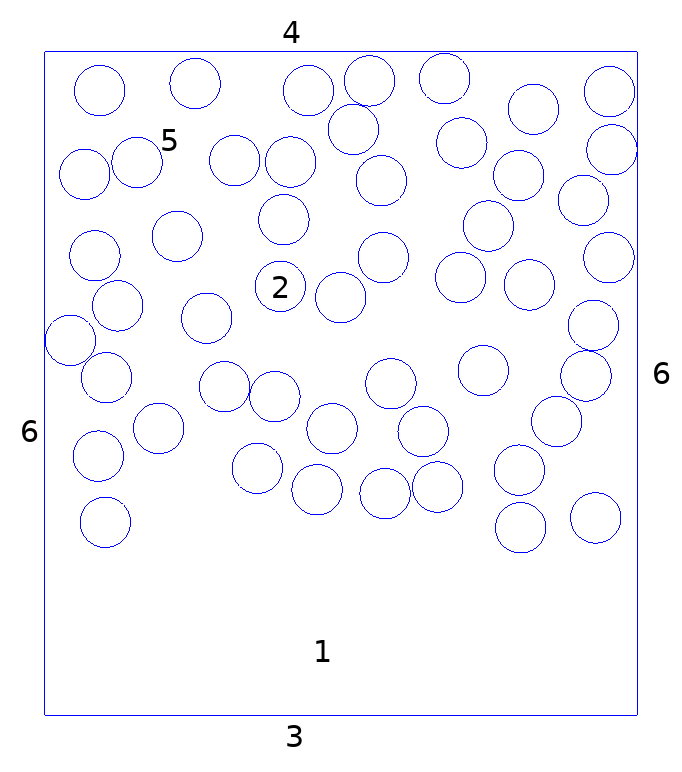
\includegraphics[width=0.5\linewidth]{pic/geometry.png}
\end{figure}

\section{Model Equations}
Taken from~\cite{garcia05}:
\begin{IEEEeqnarray*}{cc}
 1\&2 & \left\{\begin{aligned}\pn = \dv{D(\n) \nabla \n} +
  \dv{\frac{D(\n) z(x) \F \n}{R T} \nabla \phi} \\
0 = \frac{\partial\rho}{\partial{}t} =
  \dv{\kappa_T(x) \nabla \phi} + \dv{\frac{D(\n) z(x) \F \n}{R T} \nabla \n} \\
  \end{aligned}\right. \\
  3\&5 & J \cdot \nv = i_0(\n) \frac{(\alpha_a + \alpha_c) \F \eta_e(\phi, \n)}{RT}
  \\
  3 & N^0_{\Li} \cdot \nv_a = \frac{I_0}{A \F} \\
  4 &\left\{\begin{aligned}J \cdot \nv_c = - \frac{I_0}{A} \\ N_{\Li} \cdot \nv_c = 0\end{aligned}\right.\\
  6 & \left\{\begin{aligned}J \cdot \nv = 0 \\ N_{\Li} \cdot \nv = 0\end{aligned}\right.
\end{IEEEeqnarray*}

Further relations and equations:
\[J = \kappa E = - \kappa \nabla \phi\]
\[D_{\Li} = D_{\Li}^*\left(1+\frac{\partial{}\ln{\gamma_{\Li}}}{\partial{}\ln{\n}}\right)\]
\[i_0(\n) = \F k_r (n_s - \n)^{\alpha_a}(\n)^{\alpha_c}\]
\[\eta_e = E \cdot \delta - \left[ U(\n) - \Po \right]\]
\[\Po = R_cI_0\]

\subsection{Open-circuit potentials}
\begin{itemize}
  \item \ce{Li_yMn_2O_4} equation (A-1) from~\cite{doyle95} Appendix 3-A.
    \begin{IEEEeqnarray*}{rCl}
      U(y) &=& 4.19829 + 0.0565661 \tanh{[-14.5546 y + 8.60942]} \\
      &-& 0.0275479 \left[ \frac{1}{(0.998432-y)^{0.492465}}-1.90111 \right]\\
      &-& 0.157123 \exp{(-0.04738 y^8)} + 0.810239 \exp{[-40(y-0.133875)]}
      \qquad 0 \leq y \leq 1.0 \\
    \end{IEEEeqnarray*}

  \item \ce{Li_xC_6} equation (A-2) from~\cite{doyle95} Appendix 3-A.
    \[ U(x) = -0.16 + 1.32 \exp{(-3.0 x)}, \quad 0 \leq x \leq 0.7\]

\end{itemize}

\section{Variational Formulation}

\begin{IEEEeqnarray*}{rCl}
  \I{\pn v} &=& \I{\dv{D(\n) \nabla \n} v}
  +\I{\dv{\frac{D(\n) z(x) \F \n}{RT} \nabla \phi} v} \\
&=& -\I{D(\n) \nabla \n \cdot \nabla v} + \Ib{D(\n)(\nabla\n \cdot \nv) v} \\
&&-\I{\frac{D(\n) z(x) \F \n}{R T} \nabla \phi \cdot \nabla v}
+\Ib{\left(\frac{D(\n) z(x) \F \n}{R T} \nabla \phi \cdot \nv\right) v} \\
&=& -\I{D(\n) \nabla \n \cdot \nabla v}
+ \int_{\partial\Omega_{3}}{D(\n)\left(\frac{I_0}{A\F}\right) v}\ds \\
&&-\I{\frac{D(\n) z(x) \F \n}{R T} \nabla \phi \cdot \nabla v} \\
&&-\int_{\partial\Omega_{3,5}}{i_0(\n) (\alpha_a+\alpha_c)\eta_e(\phi,\n)
  \frac{D(\n) z(x) \F^2 \n}{R^2 T^2 \kappa_T(x)}} v \ds \\
&&+\int_{\partial\Omega_4}{\frac{D(\n) z(x) \F \n I_0}{R T \kappa_T(x) A} v} \ds \\
\end{IEEEeqnarray*}

\begin{IEEEeqnarray*}{rCl}
0 &=& - \I{\kappa_T(x) \nabla \phi \cdot \nabla \psi} +
\Ib{(\kappa_T(x) \nabla \phi \cdot \nv) \psi} \\
&& - \I{\frac{D(\n) z(x) \F \n}{R T} \nabla \n \cdot \nabla \psi} +
\Ib{\left(\frac{D(\n) z(x) \F \n}{R T} \nabla \n \cdot \hat{n}\right) \psi} \\
&=& - \I{\kappa_T(x) \nabla \phi \cdot \nabla \psi}
-\int_{\partial\Omega_{3,5}} i_0(\n)
\frac{(\alpha_a+\alpha_c)\F\eta_e(\phi,\n)}{RT}\psi \ds \\
&& +\int_{\partial\Omega_4} \frac{I_0}{A}\psi \ds \\
&& - \I{\frac{D(\n) z(x) \F \n}{R T} \nabla \n \cdot \nabla \psi}
+ \int_{\partial\Omega_{3}}{\frac{D(\n)I_0 z(x)\n}{RTA} \psi}\ds \\
\end{IEEEeqnarray*}

\section{Time Stepping}
The whole discretized system can be written in a short form as
\[ M \frac{\partial{}u}{\partial{}t} = f(u) \]
where $f$ is nonlinear and $M$ is the mass matrix.
We first try the Crank-Nicolson method, because it is unconditionally stable.
Another choice would be the implicit Euler method.
\[ M(u_{n+1} - u_n) = \frac{\Dt}{2} (f(u_{n+1}) + f(u_n))\]
To solve this with Newton's Method we rearrange the equation to one side
\[ 0 = \frac{\Dt}{2} (f(u_{n+1}) + f(u_n)) - M (u_{n+1} - u_n)\]
where the right-hand side has the following derivative with respect to $u_{n+1}$:
\[ \frac{\Dt}{2} \frac{\dif{}f}{\dif{}u} - M\]

Now one whole time step looks like:
\begin{algorithm}
  \begin{algorithmic}
    \STATE $w_0 = u_n$
    \STATE $i = 0$
    \WHILE{$i <$ iterations}
        \STATE $w_{i+1} = w_i + \left(\frac{\Dt}{2}\frac{\dif{}f(w_i)}{\dif{}u} - M\right)^{-1}
        \left(\frac{\Dt}{2}(f(w_{i}) + f(u_n)) - M w_i + M u_n\right)$
        \STATE $i = i + 1$
    \ENDWHILE
    \STATE $u_{n+1} = w_i$
  \end{algorithmic}
\end{algorithm}

\subsection{Version 2}
Another option would be to write the system in the following form
\begin{IEEEeqnarray*}{rCl}
n_t &=& f(n) + g(n) \phi \\
0  &=& A \phi + h(n)
\end{IEEEeqnarray*}
Applying the Crank-Nicolson method we get:
\begin{IEEEeqnarray*}{rCl}
\frac{M(n(t+\Dt)-n(t))}{\Dt} &=& \frac{1}{2}(f(n(t+\Dt)) + g(n(t+\Dt))\phi(t+\Dt) +
f(n(t))+g(n(t))\phi(t)) \\
0 &=& \frac{1}{2}\left(A \phi(t+\Dt) + h(n(t+\Dt)) + A\phi(t) + h(n(t))\right)
\end{IEEEeqnarray*}
One way to solve the system would be to eliminate $\phi(t+\Dt)$ by
rearranging the second equation
  \[\phi(t+\Dt) = - A^{-1} h(n(t+\Dt)) - \phi(t) - A^{-1} h(n(t))\]
and then plugging that into the first equation.

\section{Initial Conditions}
The initial potential at the cathode is $\SI{4.2}{\volt}$ (see Table~\ref{tbl:params}).
To obtain the initial potential on the whole domain we solve Poisson's equation:
\begin{IEEEeqnarray*}{rCl}
  \nabla \cdot D &=& \rho \\
  \nabla \cdot (\varepsilon E) &=& \rho \\
  \nabla \cdot (-\varepsilon \nabla \phi) &=& \rho
\end{IEEEeqnarray*}
And for the variational formulation we have:
\begin{IEEEeqnarray*}{rCl}
\I{\nabla \cdot (-\varepsilon \nabla \phi) \psi} &=& \I{\rho \psi} \\
\I{\varepsilon \nabla \phi \cdot \nabla \psi} -
\Ib{\varepsilon (\nabla \phi \cdot \nv) \psi} &=& \I{\rho \psi} \\
\end{IEEEeqnarray*}

\begin{table}
  \centering
  \caption{Parameters and Constants}
  \label{tbl:params}
\begin{tabular}{c|c|S|s}
  Symbol & Name & \text{Value} & Unit \\
 \hline
  $\F$ & Faraday constant & 96485.33289 & \coulomb  \mol^{-1}\\
  $R$ & molar gas constant & 8.3144598 & \J \K^{-1} \mol^{-1}\\
  $\varepsilon_0$ & vacuum permittivity & 8.85e-12 & \farad \m^{-1} \\
 \hline
  $D_{m}$ & diffusivity of electrolyte/carbon mixture & 2.66e-5& \cm^2\s^{-1} \\
  $D_{p}$ & diffusivity of \ce{Li_yMn_2O_4} particles & 1e-9& \cm^2\s^{-1} \\
  $\kappa_{T, m}$ & electric conductivity of electrolyte/carbon mixture & 2.53e-2 & \siemens\cm^{-1}\\
  $\kappa_{T, p}$ & electric conductivity of \ce{Li_yMn_2O_4} particles & 3.8e-2 & \siemens\cm^{-1}\\
  $T$ & absolute temperature & 298.15 & \K \\
  $n_T$ & normalization concentration value for lithium & 22.86 & \mol\dm^{-3} \\
  $\alpha_a$ & anodic empirical constant & 0.5 & \\
  $\alpha_c$ & cathodic empirical constant & 0.5 & \\
  $A$ & battery cross-sectional area & 24.0 & \cm^2 \\
  $k_r$ & reaction rate constant at particle/electrolyte interface & 5e-5 & \cm\s^{-1} \\
  $C$ & battery capacity & 2 & \mA\hour\cm^{-2} \\
  $n_s$ & solubility limit of lithium in the electrode & 22.86 & \mol\dm^{-3} \\
  $\delta_a$ & anode thickness & 250 & \um \\
  $\delta_c$ & cathode thickness & 174 & \um \\
  $\delta_s$ & separator thickness & 50 & \um \\
  $R_c$ & total electrode contact resistance & 2e-3 & \ohm \\
 \hline
  $n_0^c$ & normalized initial concentration of lithium in cathode & 0.18 & \\
  $\phi_0$ & initial electric potential in cathode & 4.2 & \V \\
  $I_0$ & discharge current & $x \cdot C$ & \mA\hour \\
  $\rho$ & charge density & & \coulomb \m^{-3}
\end{tabular}
\end{table}


\section{Questions}
\begin{itemize}
\item Activity coefficient?

  There's a difference between molal and molar coefficient! Which one is applicable?
  See~\cite{doyle95} chapter 4.
  They also used idealized versions, because measurement is hard.
  Also in~\cite{garcia05} they mention, that for pure and dilute compositions
  the activity coefficient satisfies Raoult's and Henry's law.

\item How to incorporate boundary conditions into time stepping?

  They are part of the (non-)linear functions $f, g, A, h$.

\item Are the functions dependent on the $\Li$ concentration dependent on the
  relative or absolute concentration?

  The open-circuit potentials are concentrations relative to maximum
  intercalation in the electrode.
  The other functions are absolute concentrations.

\item The open-circuit potentials are they with molar concentrations?

  See~\cite{garcia05} page 260.
  There it says, that the $y$ in \ce{Li_yMn_2O_4} corresponds to the relative
  concentration with respect to the solubility limit.

\item On boundaries $\partial\Omega_{3,5}$ is $z(x) = 0$ or $1$?

  Well depends probably on for which volume element the boundary element is evaluated.

\item What is porosity $\epsilon$ in~\cite{garcia05} Table II?

  Probably needed for stress equations.

\item How big is the process zone $\boldsymbol{\delta} = \delta \boldsymbol{\hat{n}}$?

  For now take it as $\delta_a$ for boundary condition 3 and the radius of the
  particle for boundary condition 5.

\item Should we use non-linear Butler-Volmer relation instead of linearized version?
  Or stated differently: Is $|\F \eta_e R T| \ll 1$?

\item Do we need the equations for the anode?

  Probably yes, because the Butler-Volmer relation needs to now the potential
  and concentration in the anode.

\item What is the reaction rate constant at the anode/electrolyte interface?

\item What is the solubility limit of lithium $n_s$ in the electrodes?

  Solubility limit in the cathode particles is \SI{22.86}{\mol\dm^{-3}}
  (see~\cite{garcia05} page 260).

  For anode maybe the open circuit potential for \ce{Li_xC_6} gives a clue,
  since its range is 0 at ~0.7 in graph from~\cite{doyle95} Appendix 3-A.
  Also~\cite{garcia05} says that the initial concentration of Lithium in the
  anode is \num{0.72}.
  So that could be the solubility limit too, since in a charged battery, the
  anode is probably full with Lithium.

\item Which open-circuit potentials should we use? Appendix 2-A or 3-A?

  I think it doesn't matter.
  It seems, like they are just measured against a different reference potential.

\item What is the initial concentration in the electrolyte?

  From pictures in~\cite{garcia05} it seems, like initial concentration of $\Li$
  is \num{1.2} in electrolyte.

\item What is the initial potential?

  In~\cite{garcia05} is mentioned that the initial potential \textbf{in} the
  cathode is \SI{4.2}{\volt} and that the cathode is short-circuit.
  What is meant with in the cathode?
  Only in the particles or also in the electrolyte which is part of the cathode?

\item How wide is the battery cell?

\item How to properly use potential / electrical field at process zone?
  How to implement in NGSolve?

  Use special normal vector coefficient function!

\item Do we need to solve equations in anode too and set each time the concentration there?

  We do not need to compute the concentration in the anode, because the normal
  electric field is properly defined by the potential in the domain.

\item What is $\varepsilon_r$ in the particles and the electrolyte?

\item What is $\rho$ in the domains?

  I would say it's 0 anyway in the particles, because the ions are only in the electrolyte.
  Otherwise we have a positive elementary charge for each Lithium-ion.
  So the charge density should be $\rho = \n \F$.

\item Can we run the whole model with the normalized concentration?
  Or do we have to use the actual concentration?

  Maybe not, because it's not linear in $\n$.
  The implementation uses the actual concentration now.

\item Do we have to make the concentration 2-dimensional by dividing by the area?

  I'm unsure about this, because on the other hand integrating over 2D then
  gives us just concentration per thickness I guess.

\end{itemize}

\bibliography{model}{}
\bibliographystyle{alpha}


\end{document}